\documentclass[hyperref={pdfpagelabels=false}]{beamer}

\usepackage{lmodern}
\usepackage{polski}
\usepackage{pdfpages}
\usepackage[utf8]{inputenc}
\usepackage{graphicx}
\usepackage{subfig}
\usetheme{Dresden}
\usecolortheme{beaver}

\author{Piotr Joński}

\title{System zarządzania projektami dedykowany metodyce Scrum}
\institute[Uniwersytet]{
	\inst{}
	Uniwersytet Zielonogórski\\
	\and
	\inst{}
	Wydział Informatyki, Elektrotechniki i Automatyki\\
	\and	
	\inst{}
	Informatyka, Sieciowe Systemy Informatyczne
	\and
	\inst{}
	Promotor dr inż. Andrzej Marciniak
}

\begin{document}
\begin{frame}	
	\titlepage
\end{frame}

\begin{frame}
	\frametitle{Agenda}
	\tableofcontents
\end{frame}

\section{Wstęp}
\begin{frame}
	\frametitle{Wstęp}
	Celem pracy był projekt oraz implementacja systemu do zarządzania projektami.
	System dedykowany jest metodyce Scrum, która jest jedną z najbardziej popularnych metod wytwarzania oprogramowania.
\end{frame}

\section[Scrum]{Czym jest metodyka Scrum}
\begin{frame}
	\frametitle{Czym jest metodyka Scrum}
Scrum jest zwinną metodyką wytwarzania oprogramowania. 
Jej~początki sięgają lat 80-tych.
Jej główne założenia to:
\begin{itemize}
	\item stały kontakt z klientem
	\item zamiana dokumentacji na implementację
	\item iteracyjne i przyrostowe wytwarzanie oprogramowania (sprint)
	\item implementacje oparte są o historyjki
	\item jak najszybsze rozwiązywanie konfliktów
	\item codzienne spotkania (stand-up) 	
\end{itemize}

Wraz ze Scrumem idą w parze inne zwinne metodyki takie: Test Driven Development (TDD) czy Feature Driven Development (FDD).
\end{frame}

\section[Przegląd narzędzi]{Przegląd dostępnych narzędzi}
\begin{frame}
	\frametitle{Przegląd dostępnych narzędzi}
	Obecnie na rynku jest wiele narzędzi, które umożliwiają zarządzanie projektami. Wiele z nich jest dedykowane metodykom zwinnym, a w szczególności Scrumowi.
	
	Podstawowymi są:
	\begin{itemize}
		\item Jira - darmowa tylko do 10 użytkowników. Posiada wiele rozbudowanych funkcji, które nie są wymagane przez większość firm. Jeden z najdroższych systemów.
		\item Bitbucket - tylko hosting zewnętrzny. Prywatne repozytoria do 5 osób. Prosty w obsłudze. Uboga funkcjonalność w porównaniu do Jiry.
		\item GitHub Issue Tracker - darmowy tylko dla projektów o otwartym kodzie źródłowym. Tylko podstawowa funkcjonalność.
	\end{itemize}
\end{frame}

\section[Cel pracy]{Cel i zakres pracy}
\begin{frame}
	\frametitle{Cel i zakres pracy}
		Praca w swoim zakresie obejmuje:
		\begin{itemize}			
			\item Zapoznanie się z literaturą tematu.
			\item Opracowanie założeń projektu.
			\item Spis wymagań funkcjonalnych i niefunkcjonalnych systemu.
			\item Implementacja wszystkich funkcjonalności.
			\item Przetestowanie systemu oraz usunięcie ewentualnych błędów.
		\end{itemize}
\end{frame}
\begin{frame}
	\frametitle{Wymagania niefunkcjonalne}
		\begin{itemize}
			\item Łatwość instalacji - użycie narzędzia Docker.
			\item Przejrzysty interfejs użytkownika - użycie biblioteki Primefaces.
			\item Wysoka użyteczność i zapamiętywalność - brak nadmiarowej funkcjonalności - implementacja tylko
			obligatoryjnych funkcji tego typu systemu.
		\end{itemize}
\end{frame}

\section{Analiza biznesowa}
\begin{frame}
	\frametitle{Analiza biznesowa}
	Metodyka Scrum definiuje wymagania funkcjonalne  w postaci tzw.
	historyjek użytkownika, które mogą mieć wiele postaci, z których w pracy wykorzystano następujące dwie:
	\item Jako \textit{\textless typ użytkownika\textgreater} mogę \textit{\textless nazwa zadania\textgreater}.
	\item Jako \textit{\textless typ użytkownika\textgreater} mogę \textit{\textless nazwa zadania\textgreater} w celu \textit{\textless cel\textgreater}.	
	
	Przykłady historyjek:
	\begin{itemize}
		\item Jako administrator mogę tworzyć nowych użytkowników w celu dodania ich do systemu.
		\item Jako administrator mogę dodawać i usuwać użytkowników z grup w celu modyfikacji zespołu.
	\end{itemize}
\end{frame}
\begin{frame}
	\frametitle{Analiza biznesowa cd.}
	\begin{figure}
		\centering
		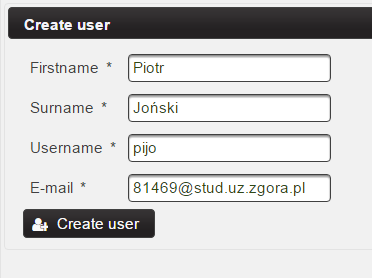
\includegraphics[width=0.7\linewidth]{user-stworz}
	\end{figure}
\end{frame}
\begin{frame}
	\frametitle{Analiza biznesowa cd.}
	\begin{figure}
	\centering
	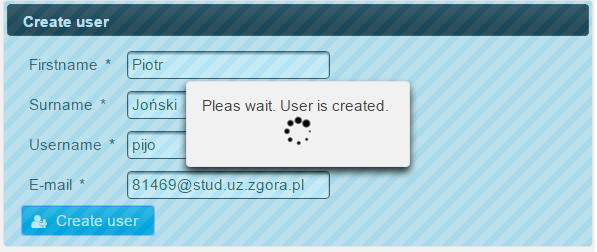
\includegraphics[width=1\linewidth]{user-czekanie}
	\end{figure}
\end{frame}
\begin{frame}
	\frametitle{Analiza biznesowa cd.}
	\begin{figure}
		\centering
		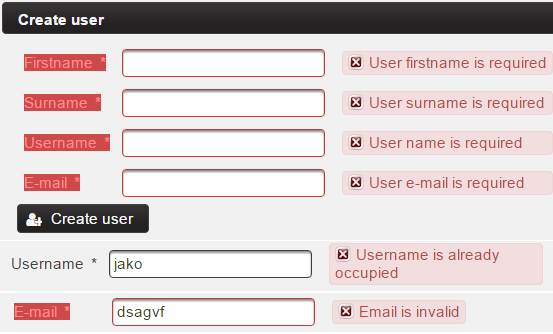
\includegraphics[width=1\linewidth]{user-blad}
	\end{figure}
\end{frame}
\begin{frame}
	\frametitle{Analiza biznesowa cd.}
	\begin{figure}
		\centering
		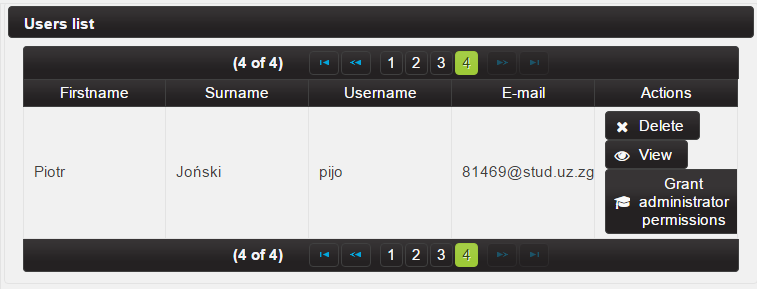
\includegraphics[width=1\linewidth]{user-list}
	\end{figure}
\end{frame}

\begin{frame}
	\frametitle{Analiza biznesowa cd.}
	\begin{figure}
		\centering
		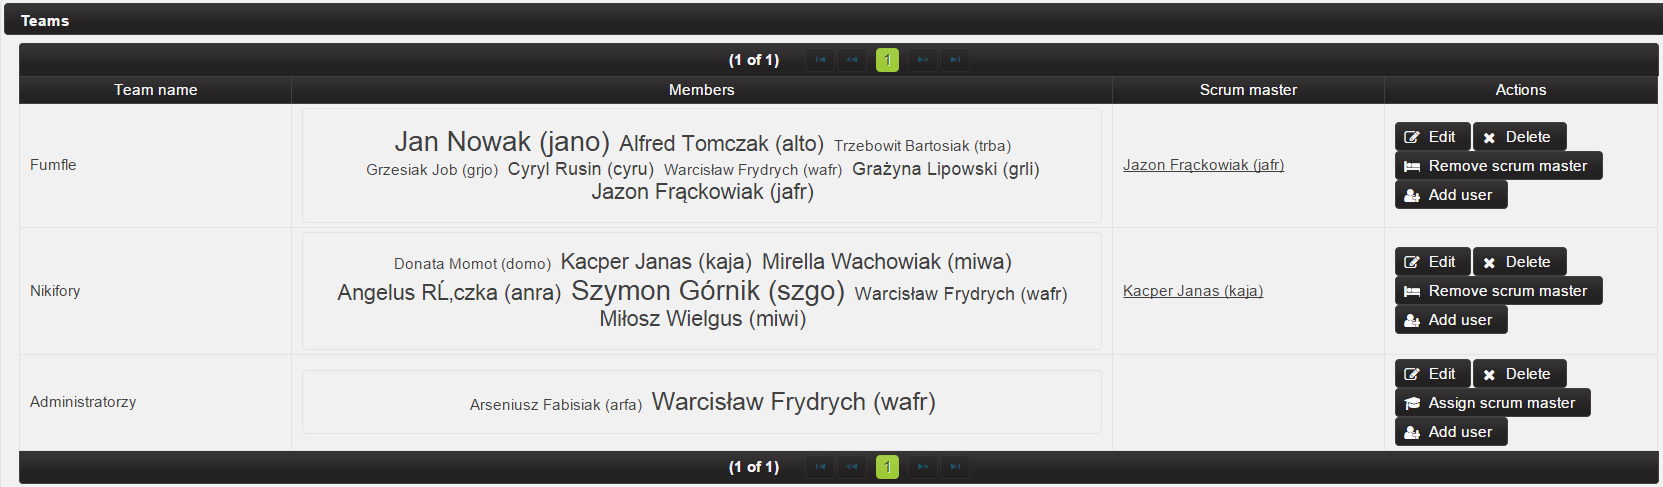
\includegraphics[height=0.5\linewidth, width=1\linewidth]{team-list}
	\end{figure}
\end{frame}
\begin{frame}
	\frametitle{Analiza biznesowa cd.}
	\begin{figure}
		\centering
		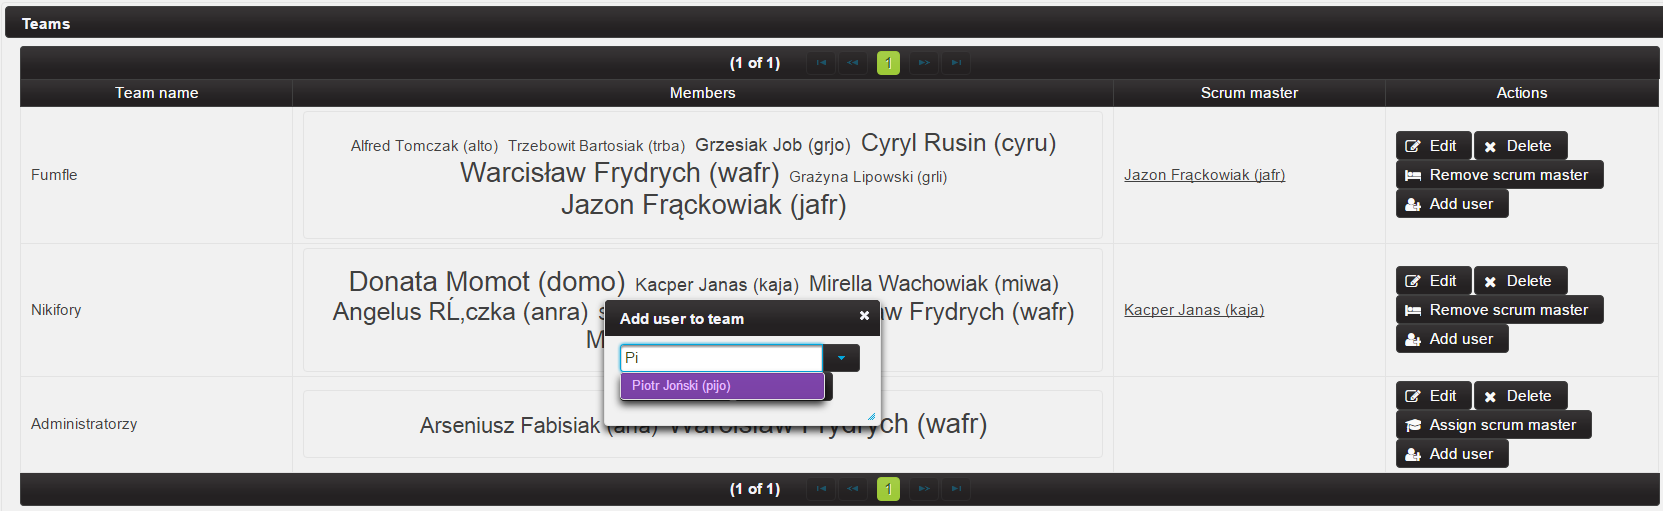
\includegraphics[height=0.5\linewidth, width=1\linewidth]{team-list-add}
	\end{figure}
\end{frame}\begin{frame}
\frametitle{Analiza biznesowa cd.}
\begin{figure}
	\centering
	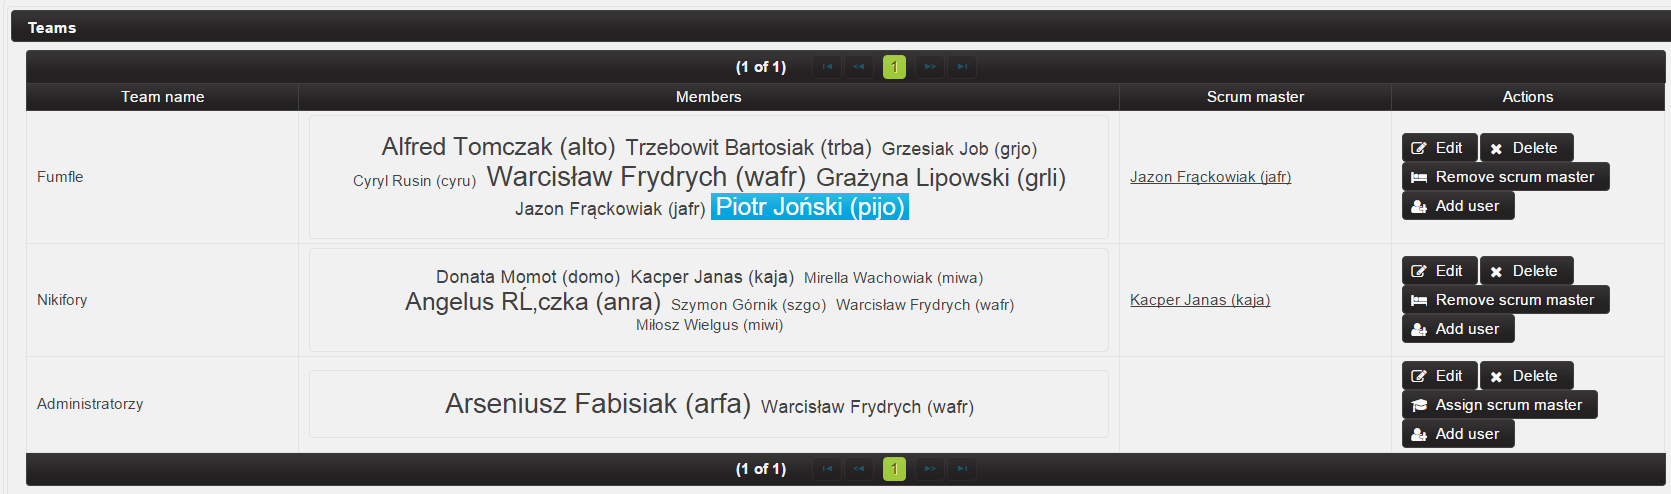
\includegraphics[height=0.5\linewidth, width=1\linewidth]{team-list-del}
\end{figure}
\end{frame}\begin{frame}
\frametitle{Analiza biznesowa cd.}
\begin{figure}
	\centering
	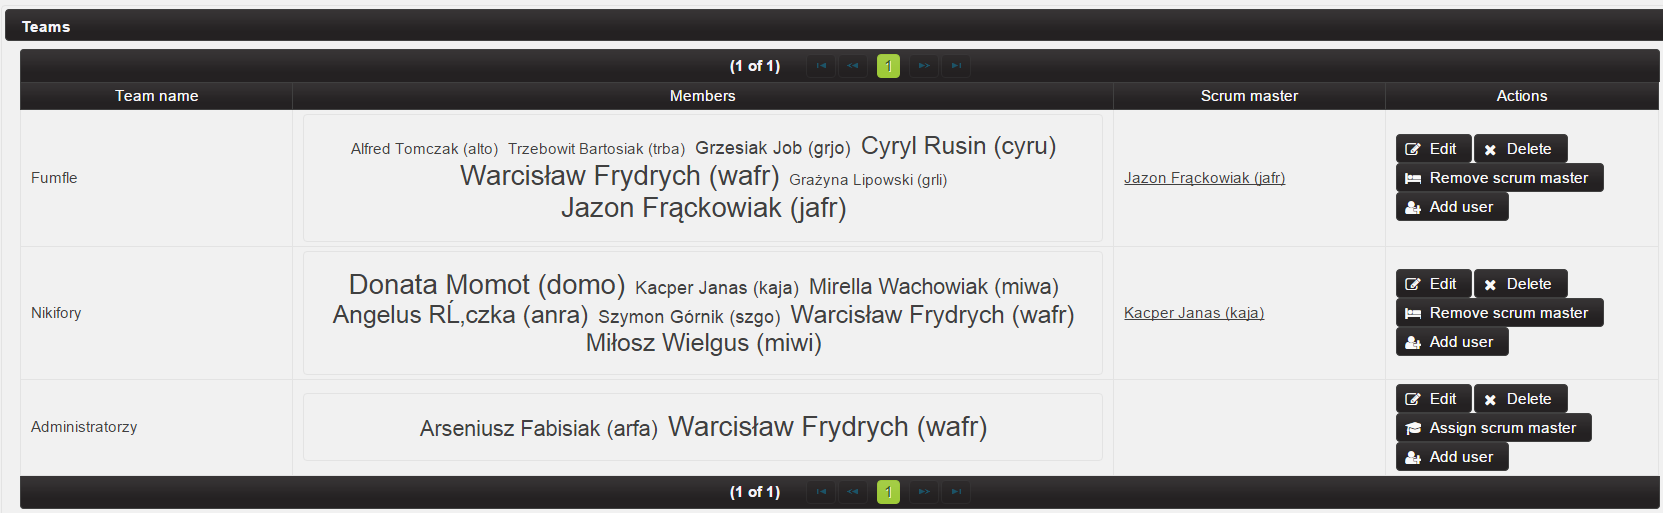
\includegraphics[height=0.5\linewidth, width=1\linewidth]{team-list-del-2}
\end{figure}
\end{frame}

\section[Diagram systemowy]{Diagram systemowy aplikacji}
\begin{frame}
	\frametitle{Diagram systemowy aplikacji}
	\begin{figure}
		\frame{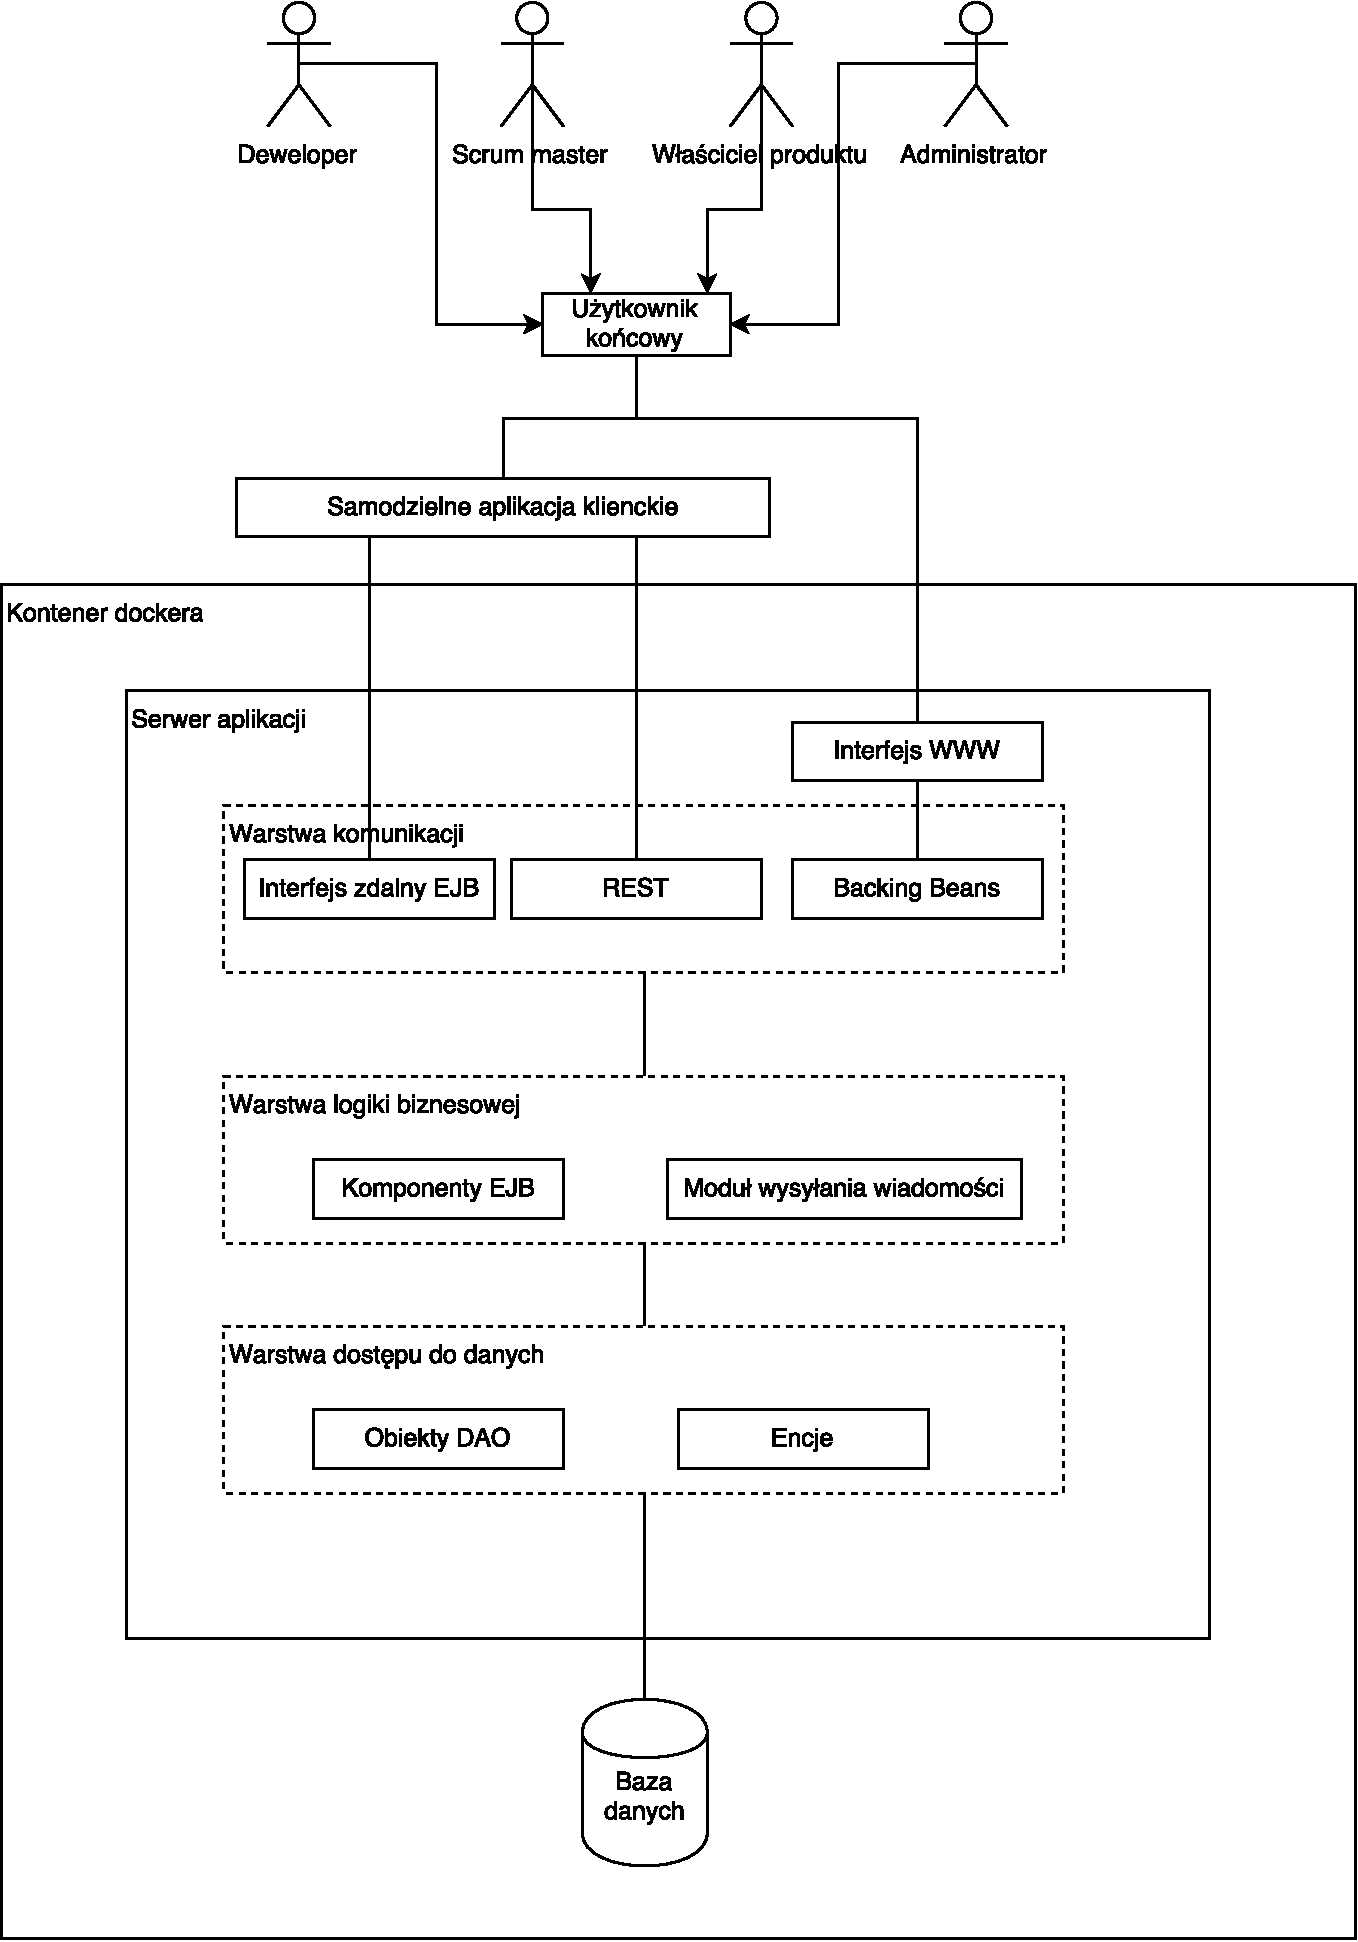
\includegraphics[page=1,height=0.6\textwidth]{diagsys.pdf}}
	\end{figure}
\end{frame}
\section[Diagram biznesowy]{Diagram jednostek biznesowych}
\begin{frame}
	\frametitle{Diagram jednostek biznesowych}
	\begin{figure}
		\frame{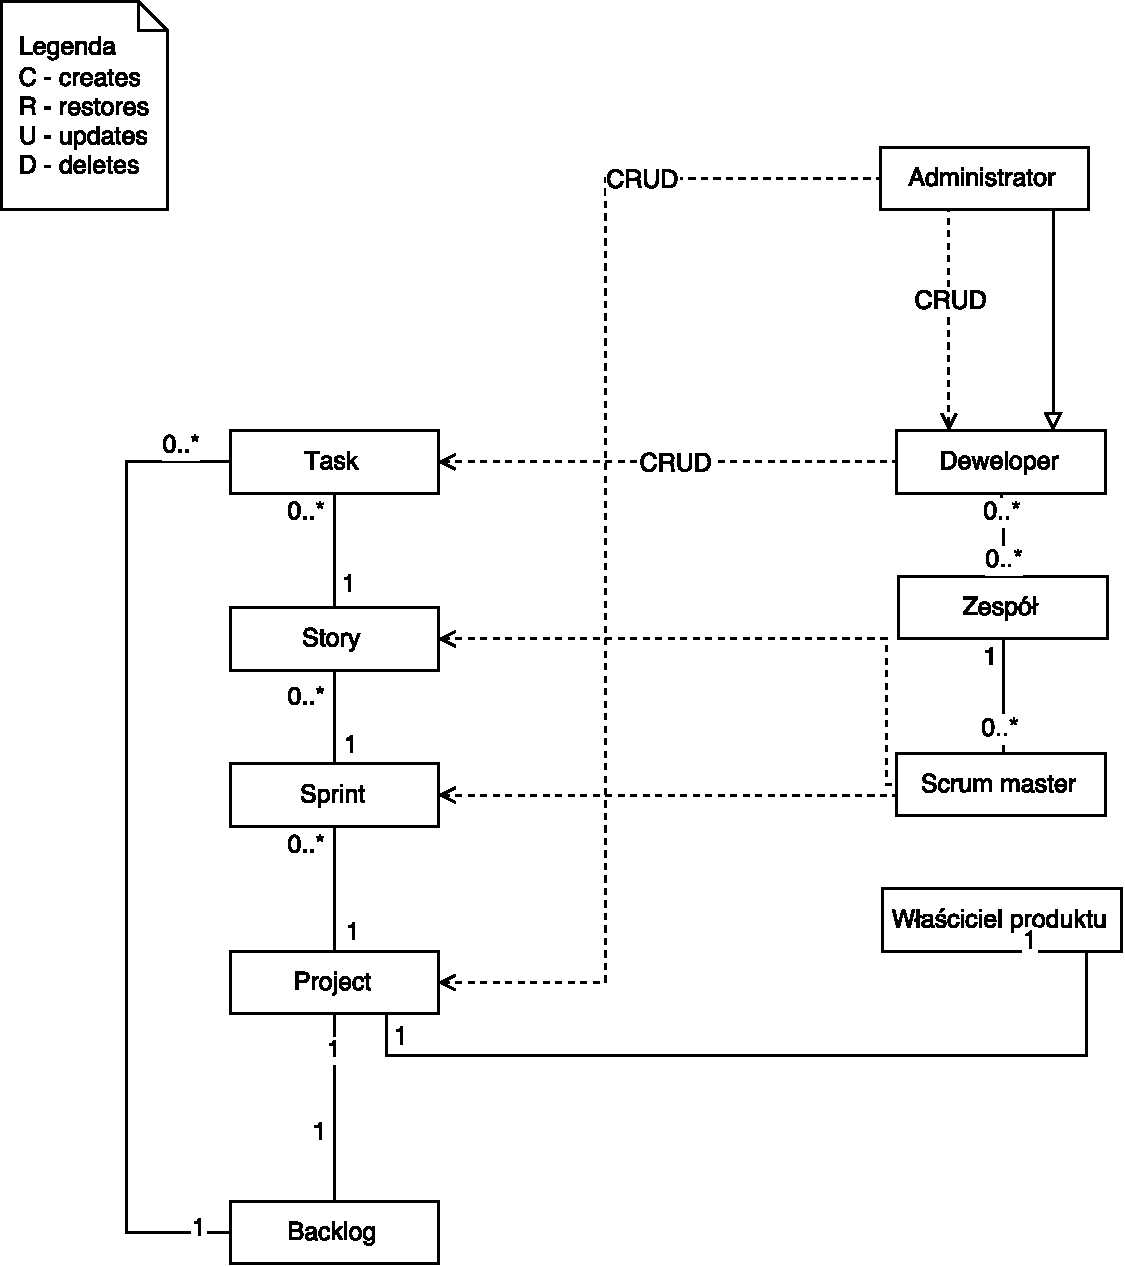
\includegraphics[page=1,height=0.6\textwidth]{diaguml.pdf}}
	\end{figure}
\end{frame}
\section{Technologie i narzędzia}
\begin{frame}
	\frametitle{Technologie i narzędzia}
	\vspace*{-1.5cm}
	\begin{figure}
		\begin{tabular}{cccc}
			\subfloat{
\includegraphics[width = 1in]{technologie/t_junit}} &
			\subfloat{
\includegraphics[width = 1in]{technologie/t_powermock}} &
			\subfloat{
\includegraphics[width = 1in]{technologie/t_arquillian}} &
			\\
			
			\subfloat{
\includegraphics[width = 1in]{technologie/ci_youtrack}} &
			\subfloat{
\includegraphics[width = 1in]{technologie/ci_intellij}} &
			\subfloat{
\includegraphics[width = 1in]{technologie/ci_github}} &
			\subfloat{
\includegraphics[width = 1in]{technologie/ci_teamcity}}\\
			
			\subfloat{
\includegraphics[width = 1in]{technologie/o_jsf}} &
			\subfloat{
\includegraphics[width = 1in]{technologie/o_primefaces}} &
			\subfloat{
\includegraphics[height = 0.4in]{technologie/o_lombok_logo}} &
			\\
			
			\subfloat{
\includegraphics[width = 1in]{technologie/w_docker}} &
			\subfloat{
\includegraphics[width = 1in]{technologie/w_postgresql}} &
			\subfloat{
\includegraphics[width = 1in]{technologie/w_wildfly}} &
			\subfloat{\includegraphics[width = 1in]{technologie/w_}}
		\end{tabular}
	\end{figure}
\end{frame}

\begin{frame}
	\begin{center}
		Dziękuję za uwagę.
		
		Czy są jakieś pytania?
	\end{center}
\end{frame}

\end{document}